%%%------------------------------------------------------------------------------------------------------------
%%% 如何度量短语的好坏
\begin{center}
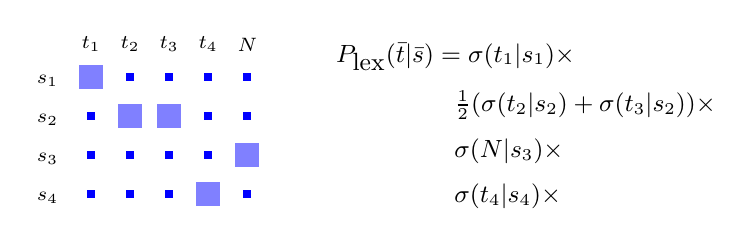
\begin{tikzpicture}

\tikzstyle{elementnode} = [rectangle,text=white,anchor=center]
\tikzstyle{srcnode} = [font=\small,anchor=south west]
\tikzstyle{tgtnode} = [left,font=\small,anchor=north east]
\tikzstyle{alignmentnode} = [rectangle,draw,minimum height=3.6*1.1cm,minimum width=0.36*1.1cm]
\tikzstyle{probnode} = [fill=blue!30,minimum width=0.4*1.1cm]
\tikzstyle{labelnode} = [above]

% alignment matrix1
\begin{scope}[scale=0.9,yshift=0.12in]
\foreach \i / \j / \c in
    {0/3/0.15, 1/3/0.15, 2/3/0.15, 3/3/0.15, 4/3/0.15,
    0/2/0.15, 1/2/0.15, 2/2/0.15, 3/2/0.15, 4/2/0.15,
    0/1/0.15, 1/1/0.15, 2/1/0.15, 3/1/0.15, 4/1/0.15,
    0/0/0.15, 1/0/0.15, 2/0/0.15, 3/0/0.15, 4/0/0.15}
    \node[elementnode,minimum size=0.6*1.1cm*\c,inner sep=0.1pt,fill=blue] (a\i\j) at (0.5*1.1cm*\i-5.4*0.5*1.1cm,0.5*1.1cm*\j-1.05*1.1cm) {};

% source
\node[srcnode] (tgt01) at (-5.9*0.5*1.1cm,-1.05*1.1cm+3.4*0.5*1.1cm) {\scriptsize{$t_1$}};
\node[srcnode] (tgt02) at ([xshift=0.5*1.1cm]tgt01.south west) {\scriptsize{$t_2$}};
\node[srcnode] (tgt03) at ([xshift=0.5*1.1cm]tgt02.south west) {\scriptsize{$t_3$}};
\node[srcnode] (tgt04) at ([xshift=0.5*1.1cm]tgt03.south west) {\scriptsize{$t_4$}};
\node[srcnode] (tgt05) at ([xshift=0.5*1.1cm]tgt04.south west) {\scriptsize{$N$}};

% target
\node[tgtnode] (src01) at (-6.0*0.5*1.1cm,-1.05*1.1cm+3.3*0.5*1.1cm) {\scriptsize{$s_1$}};
\node[tgtnode] (src02) at ([yshift=-0.5*1.1cm]src01.north east) {\scriptsize{$s_2$}};
\node[tgtnode] (src03) at ([yshift=-0.5*1.1cm]src02.north east) {\scriptsize{$s_3$}};
\node[tgtnode] (src04) at ([yshift=-0.5*1.1cm]src03.north east) {\scriptsize{$s_4$}};

% word alignment
\node[align=center,elementnode,minimum size=0.3cm,inner sep=0.1pt,fill=blue!50] (la1) at (a03) {};
\node[align=center,elementnode,minimum size=0.3cm,inner sep=0.1pt,fill=blue!50] (la2) at (a12) {};
\node[align=center,elementnode,minimum size=0.3cm,inner sep=0.1pt,fill=blue!50] (la3) at (a22) {};
\node[align=center,elementnode,minimum size=0.3cm,inner sep=0.1pt,fill=blue!50] (la4) at (a41) {};
\node[align=center,elementnode,minimum size=0.3cm,inner sep=0.1pt,fill=blue!50] (la5) at (a30) {};

\node[anchor=west] (f1) at ([xshift=3em,yshift=0.8em]a43.east) {\small{$\funp{P}_{\textrm{lex}}(\bar{t}|\bar{s})=\sigma (t_1|s_1)\times$}};
\node[anchor=north] (f2) at ([xshift=5.2em]f1.south) {\small{$\frac{1}{2}(\sigma (t_2|s_2)+\sigma (t_3|s_2))\times$}};
\node[anchor=north west] (f3) at (f2.south west) {\small{$\sigma (N|s_3)\times$}};
\node[anchor=north west] (f4) at (f3.south west) {\small{$\sigma (t_4|s_4)\times$}};

\end{scope}

\end{tikzpicture}
\end{center}